% Chapter 1

\chapter{Prediction} % Write in your own chapter title
\label{Chapter3}
\lhead{Chapter3. \emph{Prediction}} % Write in your own chapter title to set the page header

Prediction is defined as duplication of the information contained in a macro-block using previously coded data. This duplicated information is subtracted from the macro-block to form a residual. There are 2 types of prediction.

\begin{itemize}
	\item Intra-Prediction
	\item Inter-Prediction
\end{itemize}

% ref of intra+prediction paper
\subsection{Intra-Prediction}
Intra-prediction utilizes the space dependency to compress the video. The frames which are intra coded using intra-prediction are called I-frames. Following are the possible prediction modes:
\begin{itemize}
	\item \textbf{4x4 luma:} having 9 directional modes and is suitable for macro blocks that has lot of details
	\item \textbf{8x8 luma:} having 9 directional modes and is for high profiles only.
	\item \textbf{16x16 luma:} having 4 directional modes that is suitable for macro block with smoother area
	\item \textbf{8x8 chroma:} 4 possible prediction modes and used for chrominance components
\end{itemize}
In our model, 4x4 luma prediction and 8x8 chroma prediction is being implemented.

\subsubsection{4x4 Luma Prediction}
For this type of prediction, each macro block that is of \textbf{16x16} (256 pixels each of which is 8 bit wide) is divided into \textbf{4x4} block (16 pixels). Figure \ref{fig:4x4xluma} shows the reference samples for 4x4 luma prediction. 4 pixels \textbf{A,B,C,D} (adjacent to current block) of block \textbf{a}  on top of current block, pixels \textbf{E,F,G,H} of block \textbf{b} on top right corner, \textbf{I,J,K,L} of block \textbf{c} at adjacent left of current block and 1 pixel \textbf{M} of \textbf{d} block on top left corner are used for prediction of 16 pixels in the current block.

\begin{figure}[htbp]
	\centering
	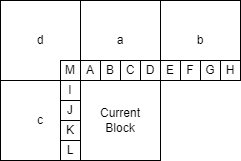
\includegraphics[width = 2.5in]{./Figures/4x4luma.png}
	\rule{35em}{0.5pt}
	\caption{Reference samples for 4x4 Luma}
	\label{fig:4x4xluma}
\end{figure}

There are total 9 prediction modes that are supported in this prediction. Major modes that are implemented in our model are as follows:

\begin{itemize}
	\item \textbf{Mode 0 (Vertical):} The predicted block is constructed by using upper samples A,B,C,D of block ‘a’ as shown in figure \ref{fig:3modes}. They are extrapolated vertically. It is suitable to predict vertical edges in the block.
	\item \textbf{Mode 1 (Horizontal):} In this mode, left samples I,J,K,L of block c are used. They are extrapolated horizontally and is suitable for horizontal edges. It can be seen in figure \ref{fig:3modes}.
	\item \textbf{Mode 2 (DC):} It utilizes average of all adjacent samples (A to D and I to L) to form the prediction of current block. It is suitable for smooth areas. Its process is shown in figure \ref{fig:3modes}.

\end{itemize}
	 
For the details of remaining modes refer to [give ref to richardson book here]. Figure \ref{fig:3modes} display the above 3 prediction modes. To create a predict sample, every color stands for a particular formula. The encoder determines each prediction direction's cost by finishing processing for all of the prediction directions, then outputs the one with the lowest cost.

\begin{figure}[htbp]
	\centering
	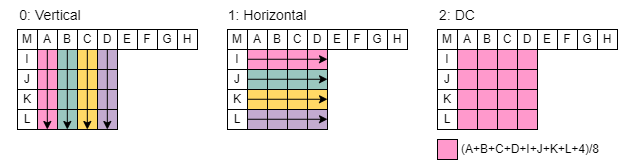
\includegraphics[width = 4in]{./Figures/3modes.png}
	\rule{35em}{0.5pt}
	\caption{Major Modes for 4x4 Luma Prediction}
	\label{fig:3modes}
\end{figure}

\subsubsection{8x8 Chroma Prediction}
This type of prediction applies on chrominance components. It is similar to 16x16 luma prediction which can be referred in [Richardson book] except the block size is 8x8 and there is different order of mode number which are:

\begin{itemize}
	\item Mode 0: DC
	\item Mode 1: Horizontal
	\item Mode 2: Vertical
	\item Mode 3: Plane
\end{itemize}

The working of first 3 modes in similar to mode 2,1,0 of 4x4 luma prediction respectively. For details of Plane mode refer to [Richardson book]. The Implemented mode in our model is DC. These modes are shown in the figure \ref{fig:8x8modes}.

\begin{figure}[htbp]
	\centering
	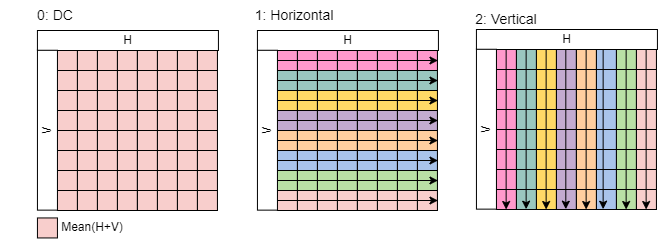
\includegraphics[width = 4in]{./Figures/8x8modes.png}
	\rule{35em}{0.5pt}
	\caption{Major Modes for 8x8 Chroma Prediction}
	\label{fig:8x8modes}
\end{figure}

\subsection{Inter-Prediction}


